\documentclass[a4paper,12pt]{article}

\usepackage[margin=1in]{geometry}
\usepackage{tikz}
\usepackage{amssymb}
\usepackage{xcolor}
\usepackage{circuitikz}
\usepackage{graphicx}

\newcommand{\ra}{$\rightarrow$}
\newenvironment{6mini}{
  \begin{minipage}{6cm}
}{
  \end{minipage}
}

\title{\texttt{Pulse Width Modulation}\\\hrulefill}
\author{Module 17}
\date{\small{12/3/2023}}

\begin{document}
    \maketitle

    \section{Pulse With Modulation}
        \textbf{Pulse Width Modulation:} Conrtolling the pulse of a digital signal for a given period
        \begin{itemize}
            \item Typically, the width of the pulse is HIGH half of the period and LOW the other half, but can changed
            \item HIGH 40\% of the period, and LOW 60\%
            \item HIGH 75\% of period, and LOW 25\%
        \end{itemize}
        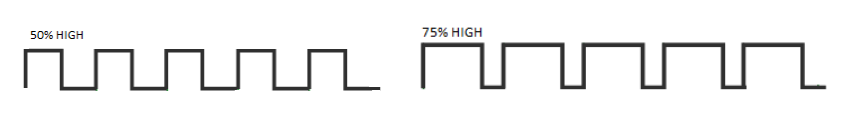
\includegraphics[width=12cm]{PWM1.png}
        \\Things that use PWMs:
        \begin{itemize}
            \item Motors
            \item Lighting for dimmer or brighter light
            \item Audio signals
        \end{itemize}
        \textbf{Duty cylce} is th epercent of the pulse HIGH compared to the period \ra~PWM is expressed as a duty cycle\\
        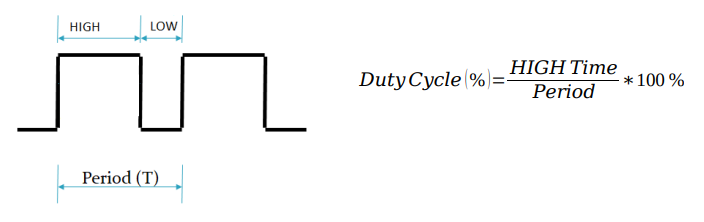
\includegraphics[width=12cm]{dutyCycle.png}
        
        \subsection{Average Voltage Value}
        A smaller duty cycle delivers an effective lower voltage value
        \begin{itemize}
            \item Motor turn slower or light appear dimmer
            \item $V_{average}=DutyCycle*V_{HIGH}$
        \end{itemize}
        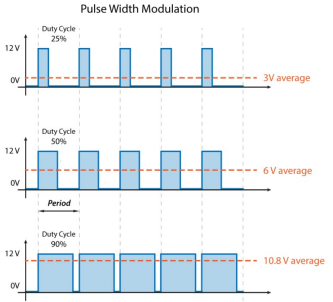
\includegraphics[width=10cm]{AVV.png}
    
    \section{Creating PWM}
    created by comparing a control to a count Value
    \begin{itemize}
        \item \texttt{Frequency:} determined by the master clock and the size of the counter
        \item \texttt{resolution:} determined b the size of the counter and the comparator
        \item \texttt{duty cycle:} determined by how the outputs of the comparator are used.
    \end{itemize}
    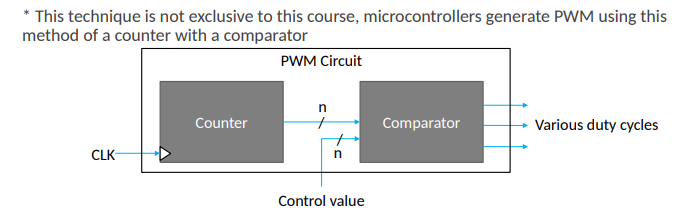
\includegraphics[width=13cm]{PMWmicro.png}
    \\ The resolution of the duty cycle is a function of the size of the counter \ra~Every change in one bit of the control value will adjust the duty cycle by the resolution. \[\textnormal{DC resolution(\%)}=\frac{1}{2^n}*100\] where n is the number of bits in counter.
    \begin{itemize}
        \item Frequency of the PWM is a function of the master clock and size of the counter.
    \end{itemize}
    \[f_{PWM}=\frac{f_{CLK}}{2^n}\] Where n is the number of bits in counter

    \subsection{PWM control Value}
    The control value is used to specify a duty cycle
    \begin{itemize}
        \item It is compared to the current count of the counter
        \item The output of the comparator will create different duty cycle \ra~ Equal $|$ Less than $|$ Greater than    
    \end{itemize}
    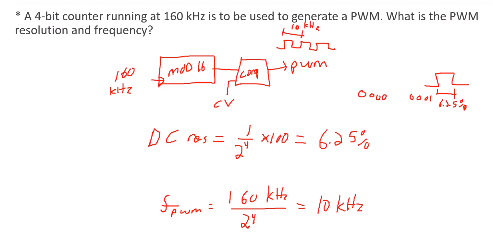
\includegraphics[width=12cm]{Ex1.png}
    \\\underline{The output of the comparator will create different duty cycle}
    \begin{itemize}
        \item Equal\ra~\(Duty~Cycle(\%)-\frac{1}{2^n}*100\)
        \item Less Than\ra~\(Duty~Cycle(\%)-\frac{Control Value}{2^n}*100\)
        \item Greater Than\ra~\(Duty~Cycle(\%)-\frac{2^n-Control~value-1}{2^n}*100\)
    \end{itemize}
    
        \subsubsection{Achieving 100\% Duty Cycle}
            \begin{itemize}
                \item OR equal and less than together
                \item \(Duty~Cylce(\%)-\frac{ControlValue+1}{2^n}*100\)
            \end{itemize}
            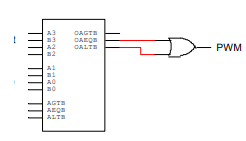
\includegraphics[width=7cm]{Achieving100Duty.png}
\end{document}